\documentclass[tikz,dvipsnames]{standalone}
\usepackage{xcolor}
\PassOptionsToPackage{dvipsnames}{xcolor}
\usepackage[utf8]{inputenc}
\usepackage{amsmath}
\usepackage{amssymb}

\usetikzlibrary{arrows,positioning,shapes}
\usetikzlibrary{decorations.pathreplacing,decorations.markings}
\usetikzlibrary{calc}
\tikzset{
  % style to apply some styles to each segment of a path
  on each segment/.style={
    decorate,
    decoration={
      show path construction,
      moveto code={},
      lineto code={
        \path [#1]
        (\tikzinputsegmentfirst) -- (\tikzinputsegmentlast);
      },
      curveto code={
        \path [#1] (\tikzinputsegmentfirst)
        .. controls
        (\tikzinputsegmentsupporta) and (\tikzinputsegmentsupportb)
        ..
        (\tikzinputsegmentlast);
      },
      closepath code={
        \path [#1]
        (\tikzinputsegmentfirst) -- (\tikzinputsegmentlast);
      },
    },
  },
  % style to add an arrow in the middle of a path
  mid arrow/.style={postaction={decorate,decoration={
        markings,
        mark=at position .5 with {\arrow[#1]{stealth}}
      }}},
  % style to add an arrow at a position of a path
  arrow at/.style 2 args={postaction={decorate,decoration={
        markings,
        mark=at position #1 with {\arrow[#2]{stealth}}
      }}},
}

\tikzset{cross/.style={cross out, draw=black, minimum size=2*(#1-\pgflinewidth), inner sep=0pt, outer sep=0pt},
%default radius will be 1pt. 
cross/.default={1pt}}

\begin{document}
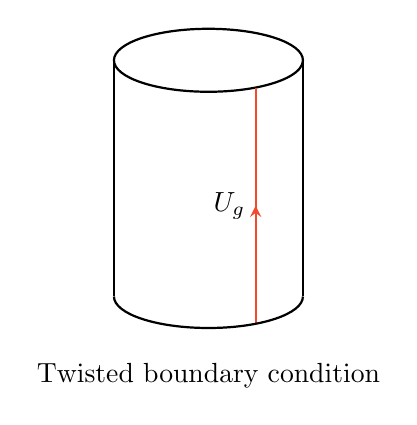
\begin{tikzpicture}[thick]
  \pgfmathsetmacro{\wid}{1.2}
  \pgfmathsetmacro{\toph}{.4}
  \pgfmathsetmacro{\hh}{3}
  \pgfmathtruncatemacro{\mrdeg}{-60}
  \draw (0,0) coordinate (ul) arc (-180:\mrdeg: {\wid} and \toph) coordinate (umr) arc(\mrdeg:0:{\wid} and \toph) coordinate (ur) arc (0:180: {\wid} and \toph);
  \draw (ul) -- ++(0,-\hh) coordinate(dl);
  \draw (ur) -- ++(0,-\hh) coordinate(dr);
  \draw (umr) ++(0,-\hh) coordinate(dmr);
  \draw[mid arrow,color=RedOrange] (dmr) -- node[midway,anchor=east,black] {$U_g$} (umr);
  \draw (dl) arc (-180:0: {\wid} and \toph);
  \coordinate (ml) at ($(ul)!.5!(dl)$);
  \node[yshift=-1cm] at ($(dl)!.5!(dr)$) {Twisted boundary condition};
\end{tikzpicture}
\end{document}
